\section{Experiments} \label{sec:experiments}
We investigate solving a Neural CDE with and without the log-ODE method on four real-world problems. Every problem was chosen for its long length. The lengths are in fact sufficiently long that adjoint-based backpropagation was used to avoid running out of memory at any reasonable batch size.

Every problem is regularly sampled, so we take $t_i = i$.

We will denote a Neural CDE model with log-ODE method, using depth $N$ and step $s$, as $\mathrm{NCDE}^s_N$. Taking $N=1$ corresponds to not using the log-ODE method as per Section \ref{subsec:tradeoff}, with data subsampled at rate $1/s$. Thus we use $\mathrm{NCDE}^1_1$ as our benchmark: no subsampling, no log-ODE method.

Each model is run three times and we report the mean and standard deviation of the test metrics along with the mean training times and memory usages. 

For each task, the hyperparameters were selected by performing a grid search on the $\mathrm{NCDE}^s_1$ model, where $s$ was chosen so that the length of the sequence was 500 steps. This was found to create a reasonable balance between training time and sequence length. (Doing hyperoptimisation on the baseline $\mathrm{NCDE}_1^1$ model would have been more difficult due to the larger training times.) 

%These hidden layer sizes were then used for the corresponding NCDE$^s_{1, 2, 3}$ models for each step length $s = 2^l, \; l \in \{0, 1, 2,..., 9\}$.

Precise details of the experiments can be found in Appendices \ref{apx:experiments} and \ref{apx:results}.

\subsection{Classification with EigenWorms}
Our first example uses the EigenWorms dataset from the UEA archive from \cite{bagnall16bakeoff}. This consists of time series of length 17,984 and 6 channels, corresponding to the movement of a roundworm. The goal is to classify each worm as either wild-type or one of four mutant-type classes.

\begin{figure}
    \centering
    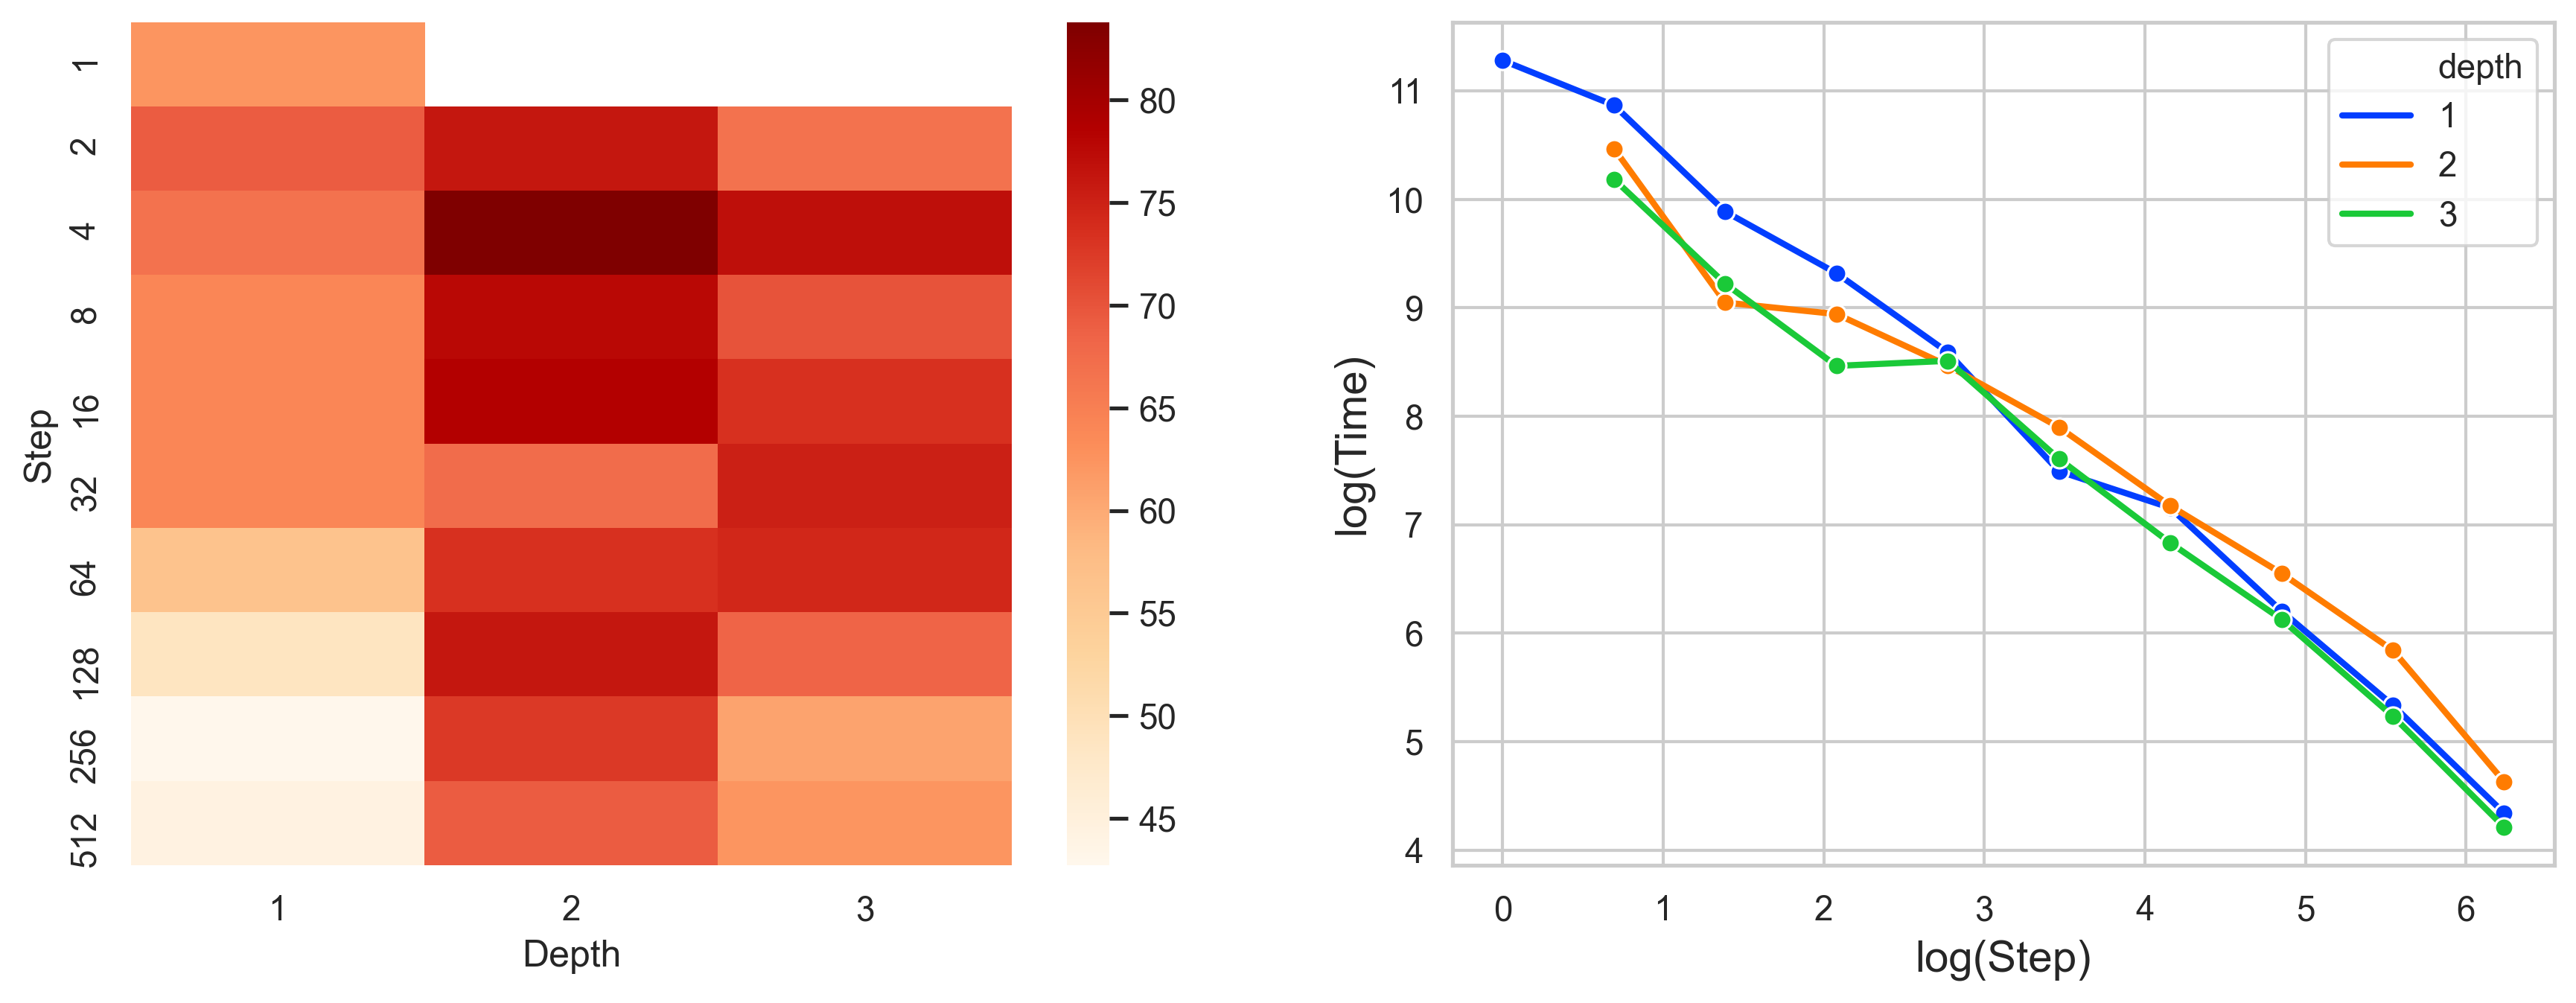
\includegraphics[width=0.95\textwidth]{Images/eigenworms.png}
    \caption{\textbf{Left:} Heatmap of accuracies on the EigenWorms dataset for differing step sizes and depths. \textbf{Right:} Log-log plot of the elapsed time of the algorithm against the step size.}
    \label{fig:eigenworms}
\end{figure}

\begin{table}[t]
    \begin{center}
        \begin{tabular}{ccccc}
        \toprule
        \textbf{Model} & \textbf{Step} & \textbf{Test Accuracy (\%)} & \textbf{Time (Hrs)} & \textbf{Memory (Mb)} \\
        \midrule
        & 1   &  62.4 $\pm$ 12.1 &          22.0 &         176.5 \\
        \multirow{2}{*}{NCDE$_1$}  & 8   &  64.1 $\pm$ 13.3 &           3.1 &          24.3 \\
        & 32  &  64.1 $\pm$ 14.3 &           0.5 &           8.0 \\
        & 128 &   48.7 $\pm$ 2.6 &           0.1 &           3.9 \\
        \midrule
        & 8   &   \textbf{77.8 $\pm$ 5.9} &           2.1 &          94.2 \\
        NCDE$_2$ & 32  &  67.5 $\pm$ 12.1 &           0.7 &          28.1 \\
          & 128 &   \textbf{76.1 $\pm$ 5.9} &           0.2 &           7.8 \\
        \hdashline\noalign{\vskip 0.5ex}
        & 8   &   70.1 $\pm$ 6.5 &           1.3 &         460.7 \\
        NCDE$_3$ & 32  &   \textbf{75.2 $\pm$ 3.0} &           0.6 &         134.7 \\
        & 128 &   68.4 $\pm$ 8.2 &           0.1 &          53.3 \\
        \bottomrule
        \end{tabular}
    \end{center}
    \caption{Performance on the UEA EigenWorms dataset for depths 1-3 and a selection of step sizes. Bold denotes that the model was the top performer for that step-size.}
    \label{tab:eigenworms}
\end{table}

See Table \ref{tab:eigenworms}. We see that the straightforward $\mathrm{NCDE}^1_1$ model takes roughly a day to train. Using the log-ODE method ($\mathrm{NCDE}_2$, $\mathrm{NCDE}_3$) speeds this up to take roughly minutes. Doing so additionally improves model performance dramatically, and reduces memory usage. Naive subsampling approaches ($\mathrm{NCDE}^{8}_1$, $\mathrm{NCDE}^{32}_1$, $\mathrm{NCDE}^{128}_1$) only achieve speedups without performance improvements.

See also Figure \ref{fig:eigenworms}, in which we summarise results for a larger range of step sizes.

\subsection{Estimating Vitals Signs from PPG and ECG Data}
Next we consider the problem of estimating vital signs from PPG and ECG data. The data is taken from the TSR archive \cite{MonashTSRegressionArchive} and involves data from the Beth Israel Deaconess Medical Centre (BIDMC). We consider three tasks whereby we aim to predict a persons respiratory rate (RR), their heart rate (HR), and their oxygen saturation (SpO2). This data is sampled at 125hZ with each series having a length of 4000, 7949 training samples, and a dimension of 3 (including time).

We train a model on each of the three vitals sign prediction tasks using a similar approach to the EigenWorms dataset. The metric used to evaluate performance is the root mean squared error (RMSE) loss which is the standard loss considered in the TSR archive. The results over a range of step sizes are presented in table (\ref{tab:bidmc}). The full results over all step sizes, along with a plots analogous to figure \ref{fig:eigenworms} are left to Appendix \ref{apx:results}.

\begin{table}[t]
    \small
    \begin{center}
        \begin{tabular}{ccccccccc}
        \toprule
        \multirow{2}{*}{\textbf{Depth}} & \multirow{2}{*}{\textbf{Step}} & \multicolumn{3}{c}{\textbf{RMSE}} & \multicolumn{3}{c}{\textbf{Time (H)}} & \multirow{2}{*}{\textbf{Memory (Mb)}} \\
        \cmidrule(lr){3-5} \cmidrule(lr){6-8}
         & & RR & HR & SpO$_2$ & RR & HR & SpO$_2$ & \\
         \midrule
        & 1   &  2.79 $\pm$ 0.04 &   9.82 $\pm$ 0.34 &  2.83 $\pm$ 0.27 &          23.8 &          22.1 &          28.1 &               56.5 \\
        \multirow{2}{*}{NCDE$_1$} & 8   &   2.80 $\pm$ 0.06 &  10.72 $\pm$ 0.24 &  3.43 $\pm$ 0.17 &           3.0 &           2.6 &           4.8 &               14.3 \\
          & 32  &  2.53 $\pm$ 0.23 &  12.23 $\pm$ 0.43 &  2.68 $\pm$ 0.12 &           1.9 &           0.9 &           2.2 &                9.8 \\
          & 128 &  2.64 $\pm$ 0.18 &  11.98 $\pm$ 0.37 &  2.86 $\pm$ 0.04 &           0.2 &           0.2 &           0.3 &                8.7 \\
        \midrule
        & 8   &  2.63 $\pm$ 0.12 &   8.63 $\pm$ 0.24 &  2.88 $\pm$ 0.15 &           2.1 &           3.4 &           3.3 &               21.8 \\
        NCDE$_2$ & 32  &   1.90 $\pm$ 0.02 &     7.90 $\pm$ 1.00 &   1.69 $\pm$ 0.20 &           1.2 &           1.1 &           2.0 &               13.1 \\
          & 128 &  1.86 $\pm$ 0.03 &   6.77 $\pm$ 0.42 &  1.95 $\pm$ 0.18 &           0.3 &           0.4 &           0.7 &               10.9 \\
        \hdashline\noalign{\vskip 0.5ex}
        & 8   &  \textbf{2.42 $\pm$ 0.19} &    \textbf{7.67 $\pm$ 0.40} &  \textbf{2.55 $\pm$ 0.13} &           2.9 &           3.2 &           3.1 &               43.3 \\
        NCDE$_3$ & 32  &  \textbf{1.67 $\pm$ 0.01} &    \textbf{4.50 $\pm$ 0.70} &  \textbf{1.61 $\pm$ 0.05} &           1.3 &           1.8 &           7.3 &               20.5 \\
          & 128 & \textbf{1.51 $\pm$ 0.08} &  \textbf{2.97 $\pm$ 0.45} &  \textbf{1.37 $\pm$ 0.22} &           0.5 &           1.7 &           1.7 &               17.3 \\
        \bottomrule
        \end{tabular}
    \end{center}
    \caption{The RMSE scores on the test set for each of the vitals signs prediction tasks (RR, HR, SpO$_2$) on the BIDMC dataset. The memory usage is given as the mean over all three of the tasks as it was approximately the same for any task for a given depth and step. The bold values denote the algorithm with the lowest test set loss for a fixed step size for each task.}
    \label{tab:bidmc}
\end{table}

We find that the depth $3$ model is the top performer for every task at any step size. Whats more, the top performing depth 3 model from each category also significantly outperforms the NCDE$^1_1$ model with a significantly reduced training time. This again illustrates that the increased step size not only reduces training time, but can also improve model performance. We believe this is attributable to the log-ODE model being better at learning these long-term dependencies, as the worst scores of the NCDE$^s_{2, 3}$ models are with step sizes 2 and 4 for all tasks where they are on par (or worse) than the corresponding depth 1 model.

Both experiments give show that the depth 2 and 3 models can not only reduce training times with similar levels of performance, but can additionally result in improved performance over these large steps. 
